\documentclass[
a4paper, 
11pt, 
ngerman,
listof=totoc,
%bibliography=totoc,
bibliography=totocnumbered
]{scrreprt}


\usepackage[T1]{fontenc}
\usepackage[utf8]{inputenc}
\usepackage[ngerman]{babel}
\usepackage{graphicx}
\usepackage{lipsum}
\usepackage{csquotes}

\usepackage[
backend=biber,
style=authoryear-ibid,
%sorting=ynt
]{biblatex}
\addbibresource{gravitropismus-bibliography.bib}

\title{Untersuchung von Gravitropismus bei \emph{Lepidium sativum} mit einem selbstgebautem Klinostat unter Zimmerbedingungen}

\subtitle{W-Seminararbeit im Fach Biologie am Luitpold-Gymnasium München}

\author{Alexandra Smirnova}

\begin{document}
\maketitle
\tableofcontents

\chapter{Gravitropismus als wichtige Pflanzeneigenschaft}



\chapter{Fachliche Analyse der Thematik: Gravitropismus}

\section{Gravitropismus}
Die Bestimmung der Wachstumrichtung der Wurzel und des Sprosses unter dem Einfluss der Schwerkraft wird als Gravitropismus (Geotropismus) bezeichnet. Dabei werden drei Bewegungen unterschieden: Positiv gravitrop, negativ gravitrop und transversalgravitrop. Positiv gravitrop bedeutet, dass das Wachstum zur Schwerkraftquelle hin (nach unten) erfolgt. Positiv gravitrope Organe wären zum Beispiel Wurzeln, Rhizoide (wurzelähnliche Strukturen), Moose oder Farnprothallien. Negativ gravitrop dagegen bedeutet, dass die Organe wie Sprossen, Sporangienträger der Schimmelpilze der Gattung Mucor oder Fruchtkörper mancher Pilze von der Schwerkraftquelle weg (nach oben) wachsen. Seitenwurzeln der ersten Ordnung (Nebenwurzeln, die von der Hauptwurzel entspringen) und zahlreiche Seitenzweige sowie Blätter wachsen transversalgravitrop: entweder flach oder quer nach unten in einem speziellen Winkel 
\parencite[449]{Strasburger}. 
Legt man eine Pflanze quer, so werden sich die Organe, Wurzeln und Spross, krümmen, bis sie senkrecht stehen und wieder positiv bzw. negativ gravitrop wachsen
\parencite[528]{Luettge}.

\section{Differenzielles Wachstum}


\section{Koordination von Gravitropismus durch Pflanzenhormone}

\chapter{Experimenteller Nachweis von Gravitropismus bei \emph{Lepidium sativum}}

\section{Methoden}

\subsection{Pflanzen}

Für das Experiment wurde die \emph{Lepidium sativum} (Kresse) genommen. Sie ist eine schnellwüchsige Pflanze und kann auf jedem lockeren, durchlässigen Gartenboden wachsen (der Firma Kiepenkerl).



\subsection{Verwendete Materialien und Geräte}
Außer den Pflanzen wurden vier gleich große Behälter und ein selbst gebautes Säckchen, eine Plastiktüte, ein Messzylinder (in ml) und Gegenstände für Stützung der Behälter (z.B. Holzklotz) verwendet. Für die Pflanzen wurden Anzucht-Quelltabs (der Firma Windhager) benutzt, da die Erde torffrei ist und Kokosfasern enthält, die dafür sorgen, dass die Feuchtigkeit besser aufgenommen wird. Dadurch können Samen schneller keimen und Wurzeln sich besser ausbilden, wodurch das Wachstum der Pflanze gefördert wird (http://www.windhager.eu/de/garten/anzucht/toepfe-quelltabs/anzucht-quelltabs-49892/). 

-Zimmerlicht, -temperatur, Wasser (jeden Tag 20ml in jeden Behälter)
-Aufnahme des ganzen Experimentes mit Kamera (Canon)

\subsubsection{Klinostat}

create blueprint with OpenSCAD or LibreCAD or (paid) Autodesk

-(Bild?)

\subsection{Versuchsbeschreibung}

\subsubsection{Vorbereitung}

\subsubsection{Durchführung}

\paragraph{7.Tag (03.06.18)} 

Neuer Versuch mit Klinostat: Start um 12:40, Ende am 9.Tag (05.06.18) um 23:45; Bemerkung: Sprossen über 3cm (Annahme, dass die Krümmung deshalb verlangsamt war); Foto 5 (kleinerer Spross gebogen, größerer Spross nur geneigt)

\subparagraph{7.Tag (03.06.18)}

Neuer Versuch mit Klinostat: Start um 12:40, Ende am 9.Tag (05.06.18) um 23:45; Bemerkung: Sprossen über 3cm (Annahme, dass die Krümmung deshalb verlangsamt war); Foto 5 (kleinerer Spross gebogen, größerer Spross nur geneigt)

\begin{itemize}
	\item 1. Tag (28.05.18): Aufbau des Experiments: alle Behälter mit der Anzuchterde gefüllt und auf der Plastiktüte (Vermeidung von Schmutz auf den Boden), Aussaat der Samen (jeweils 20 Stück in drei Behältern, gebliebene Samen in den vierten Becher (als Vergleichsergebnis gedacht), im Säckchen nur 3 Samen)
	
	\item 2. Tag (29.05.18): Keimung der Samen
	
	\item 3. Tag (30.05.18): Sprossen bis zu 2cm, noch keine Blätter, dennoch instabile Haft der Sprösslinge (noch nicht geeignet für das Experiment)
	
	\item 4. Tag (31.05.18): Gebildete Blätter, stabile Haft der Sprösslinge (geeignet für das Experiment), Säckchen bereit für den Versuch mit dem Klinostat (20 min für die Befestigung des Behälters an das Klinostat) und um 12.45 Versuch gestartet mit Geschwindigkeit 1 Umdrehung pro Minute; um 15.45 gestoppt, da die Pflanzen sich vollständig gebogen haben (nach außen die Sprossen, nach innen die Wurzeln), Foto 1 und 2
	
	\item 5. Tag (01.06.18): Über Abend Rückbildung der Pflanzen, gleicher Versuch nochmal möglich, diesmal mit genauen Zeitangaben; aber um 12:53 (des nächsten Tages) Klinostat kaputt gefunden; Pflanzen haben aber angefangen sich sichtbar zu biegen (gelaufene Zeit ca. 1 Stunde und 8 Minuten)
	
	\item 6. Tag (02.06.18): Klinostat wieder repariert (mit Uhu-Kleber), Sprossen fast bis zu 3cm  
	-dabei Beginn des zweiten Experiments: verschiedene Positionierungen der drei Behälter: 1) vertikal zu Boden 2) Kopfüber 3) gewinkelt 
	
	\item 7. Tag (03.06.18): neuer Versuch mit Klinostat: Start um 12:40, Ende am 9.Tag (05.06.18) um 23:45; Bemerkung: Sprossen über 3cm (Annahme, dass die Krümmung deshalb verlangsamt war); Foto 5 (kleinerer Spross gebogen, größerer Spross nur geneigt)
	- Krümmung sichtbar auch bei dem zweiten Versuch 
	(-zwei Bilder)
\end{itemize}

\section{Ergebnisse}

\section{Diskussion}

\chapter{Fazit und Ausblick}


\printbibliography

% afa
% \begin{figure}
% 	\centering
% 	\includegraphics[width = .5\linewidth]{images/IMG_1117.JPG}
% 	\caption{a nice little caption \label{nice_picture}}
% \end{figure}
% asd
% a
% 
% as we see in image \ref{nice_picture}
% 
% \begin{figure}
%  \centuring 
%  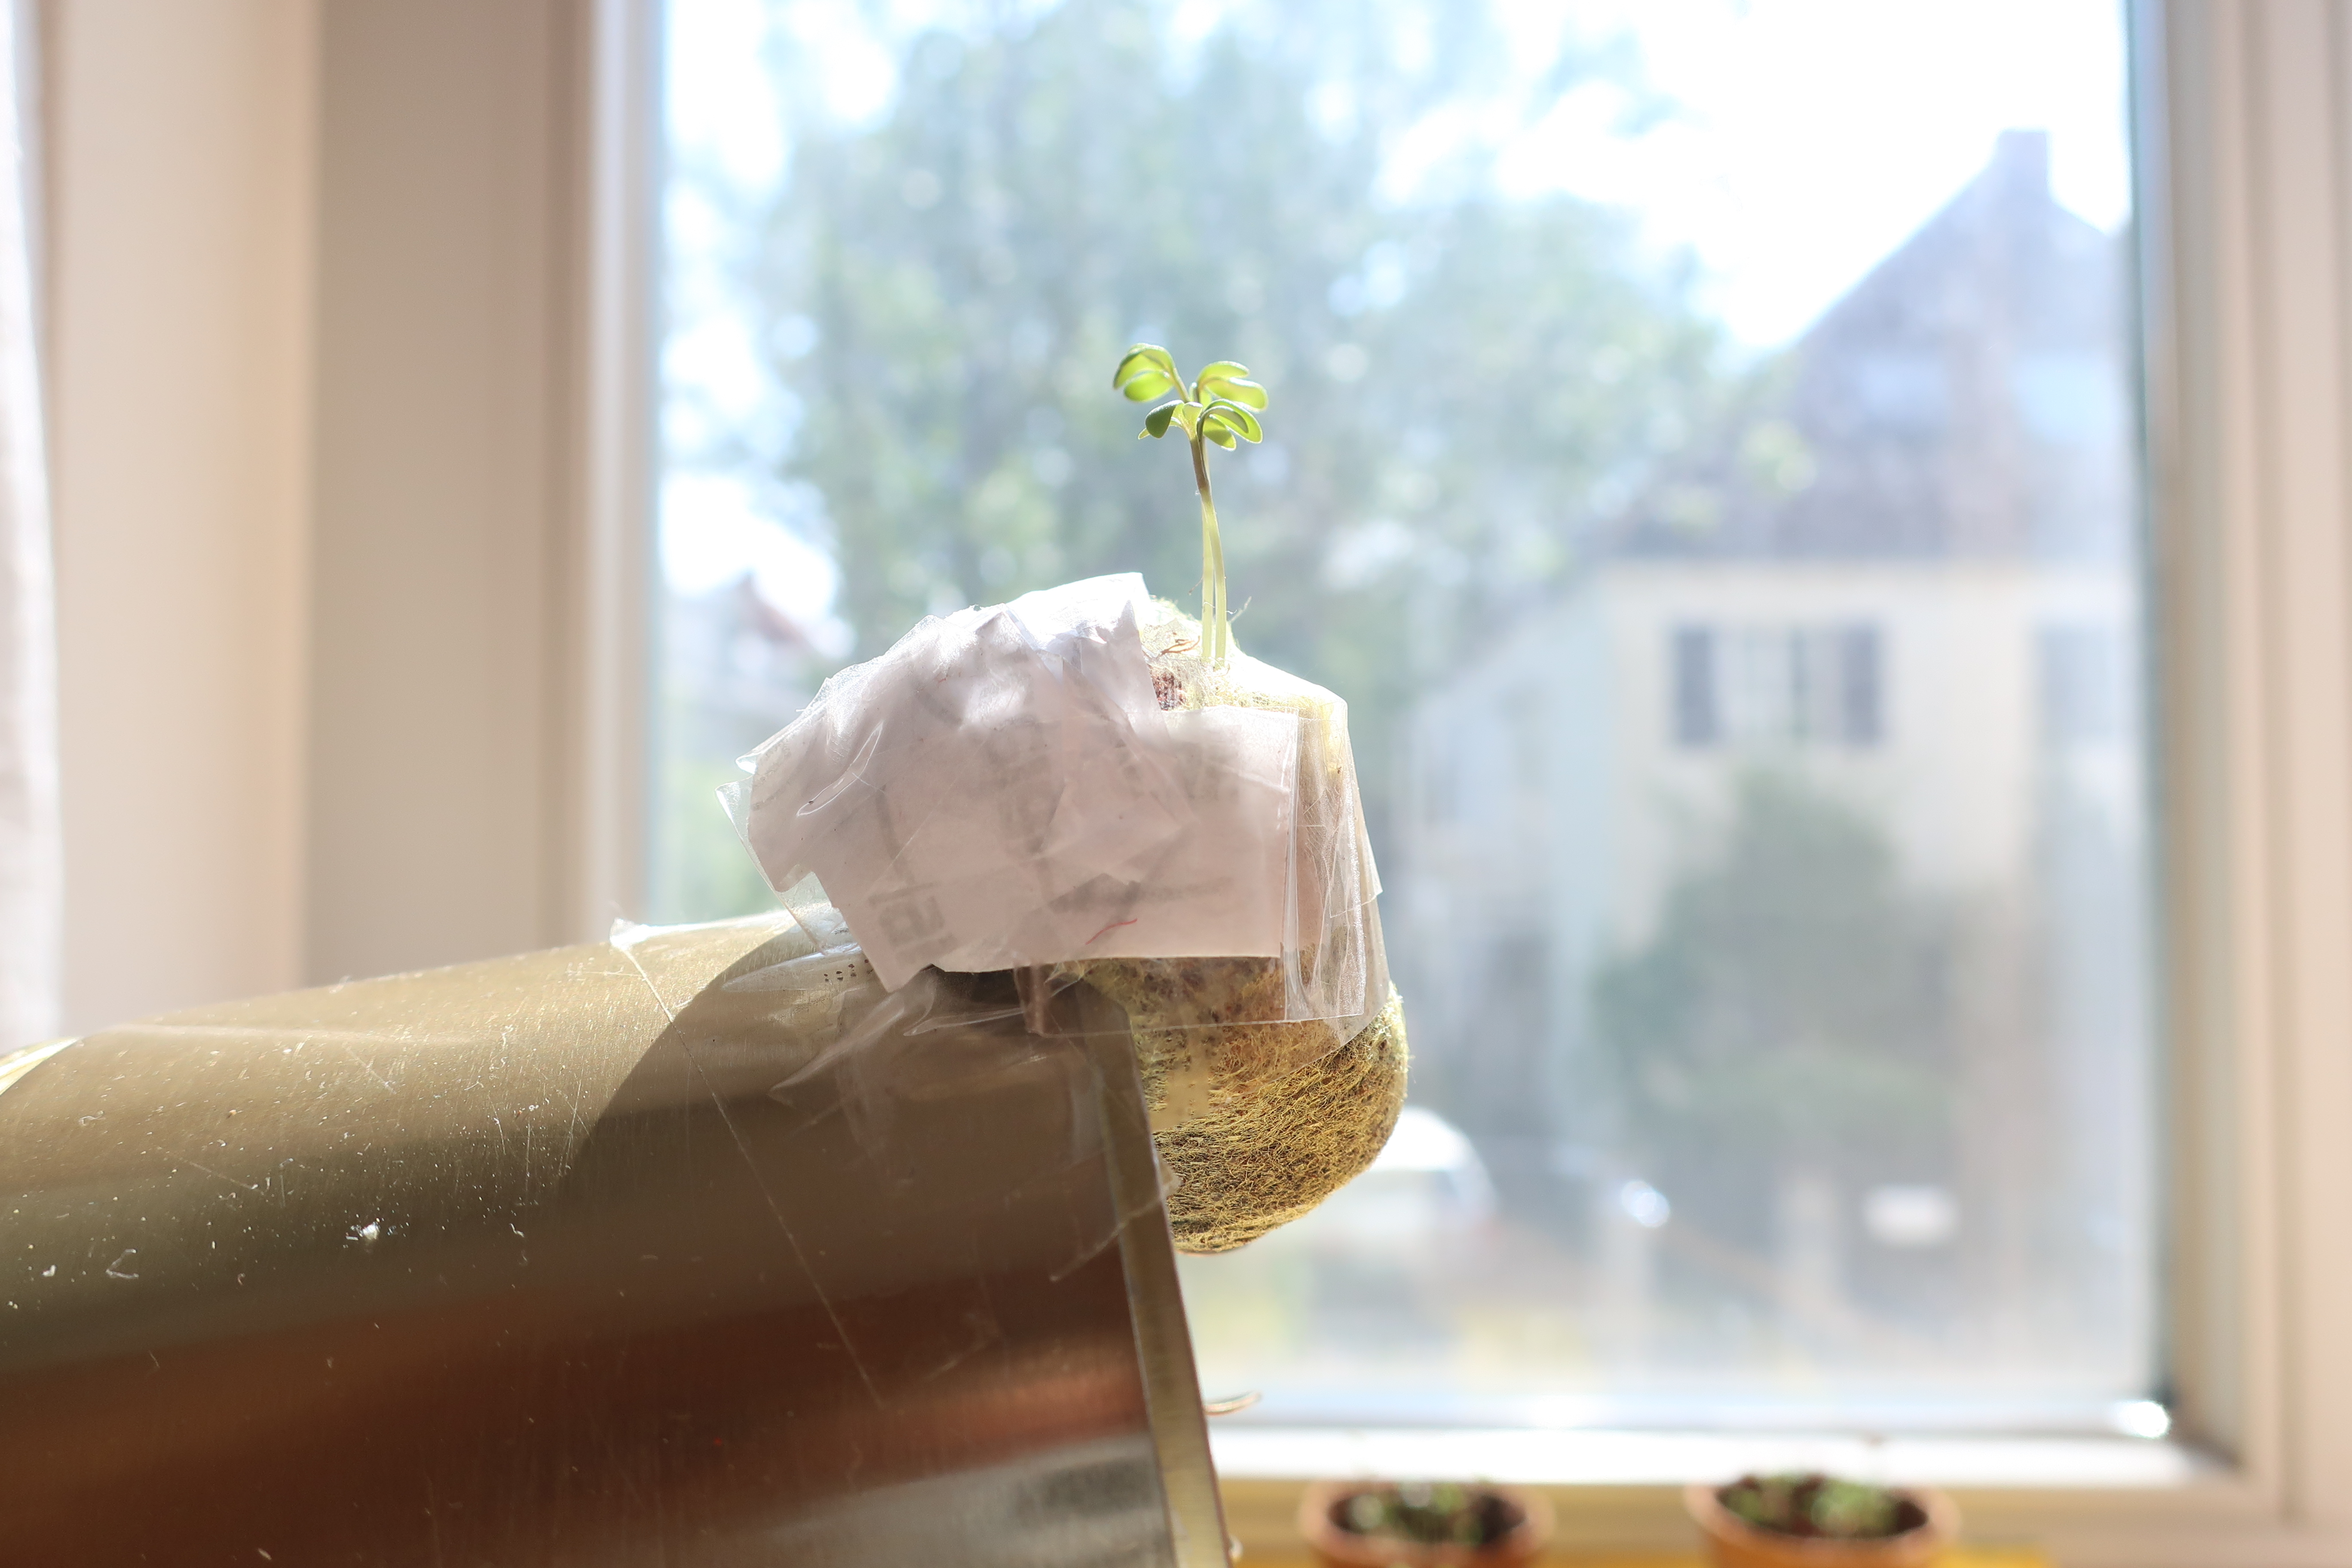
\includegraphics [width = .5\linewidth]{images/IMG_1083.JPG}
%  \end {figure} 
% Photo 1
%
% \begin{figure}
%  \centuring 
%  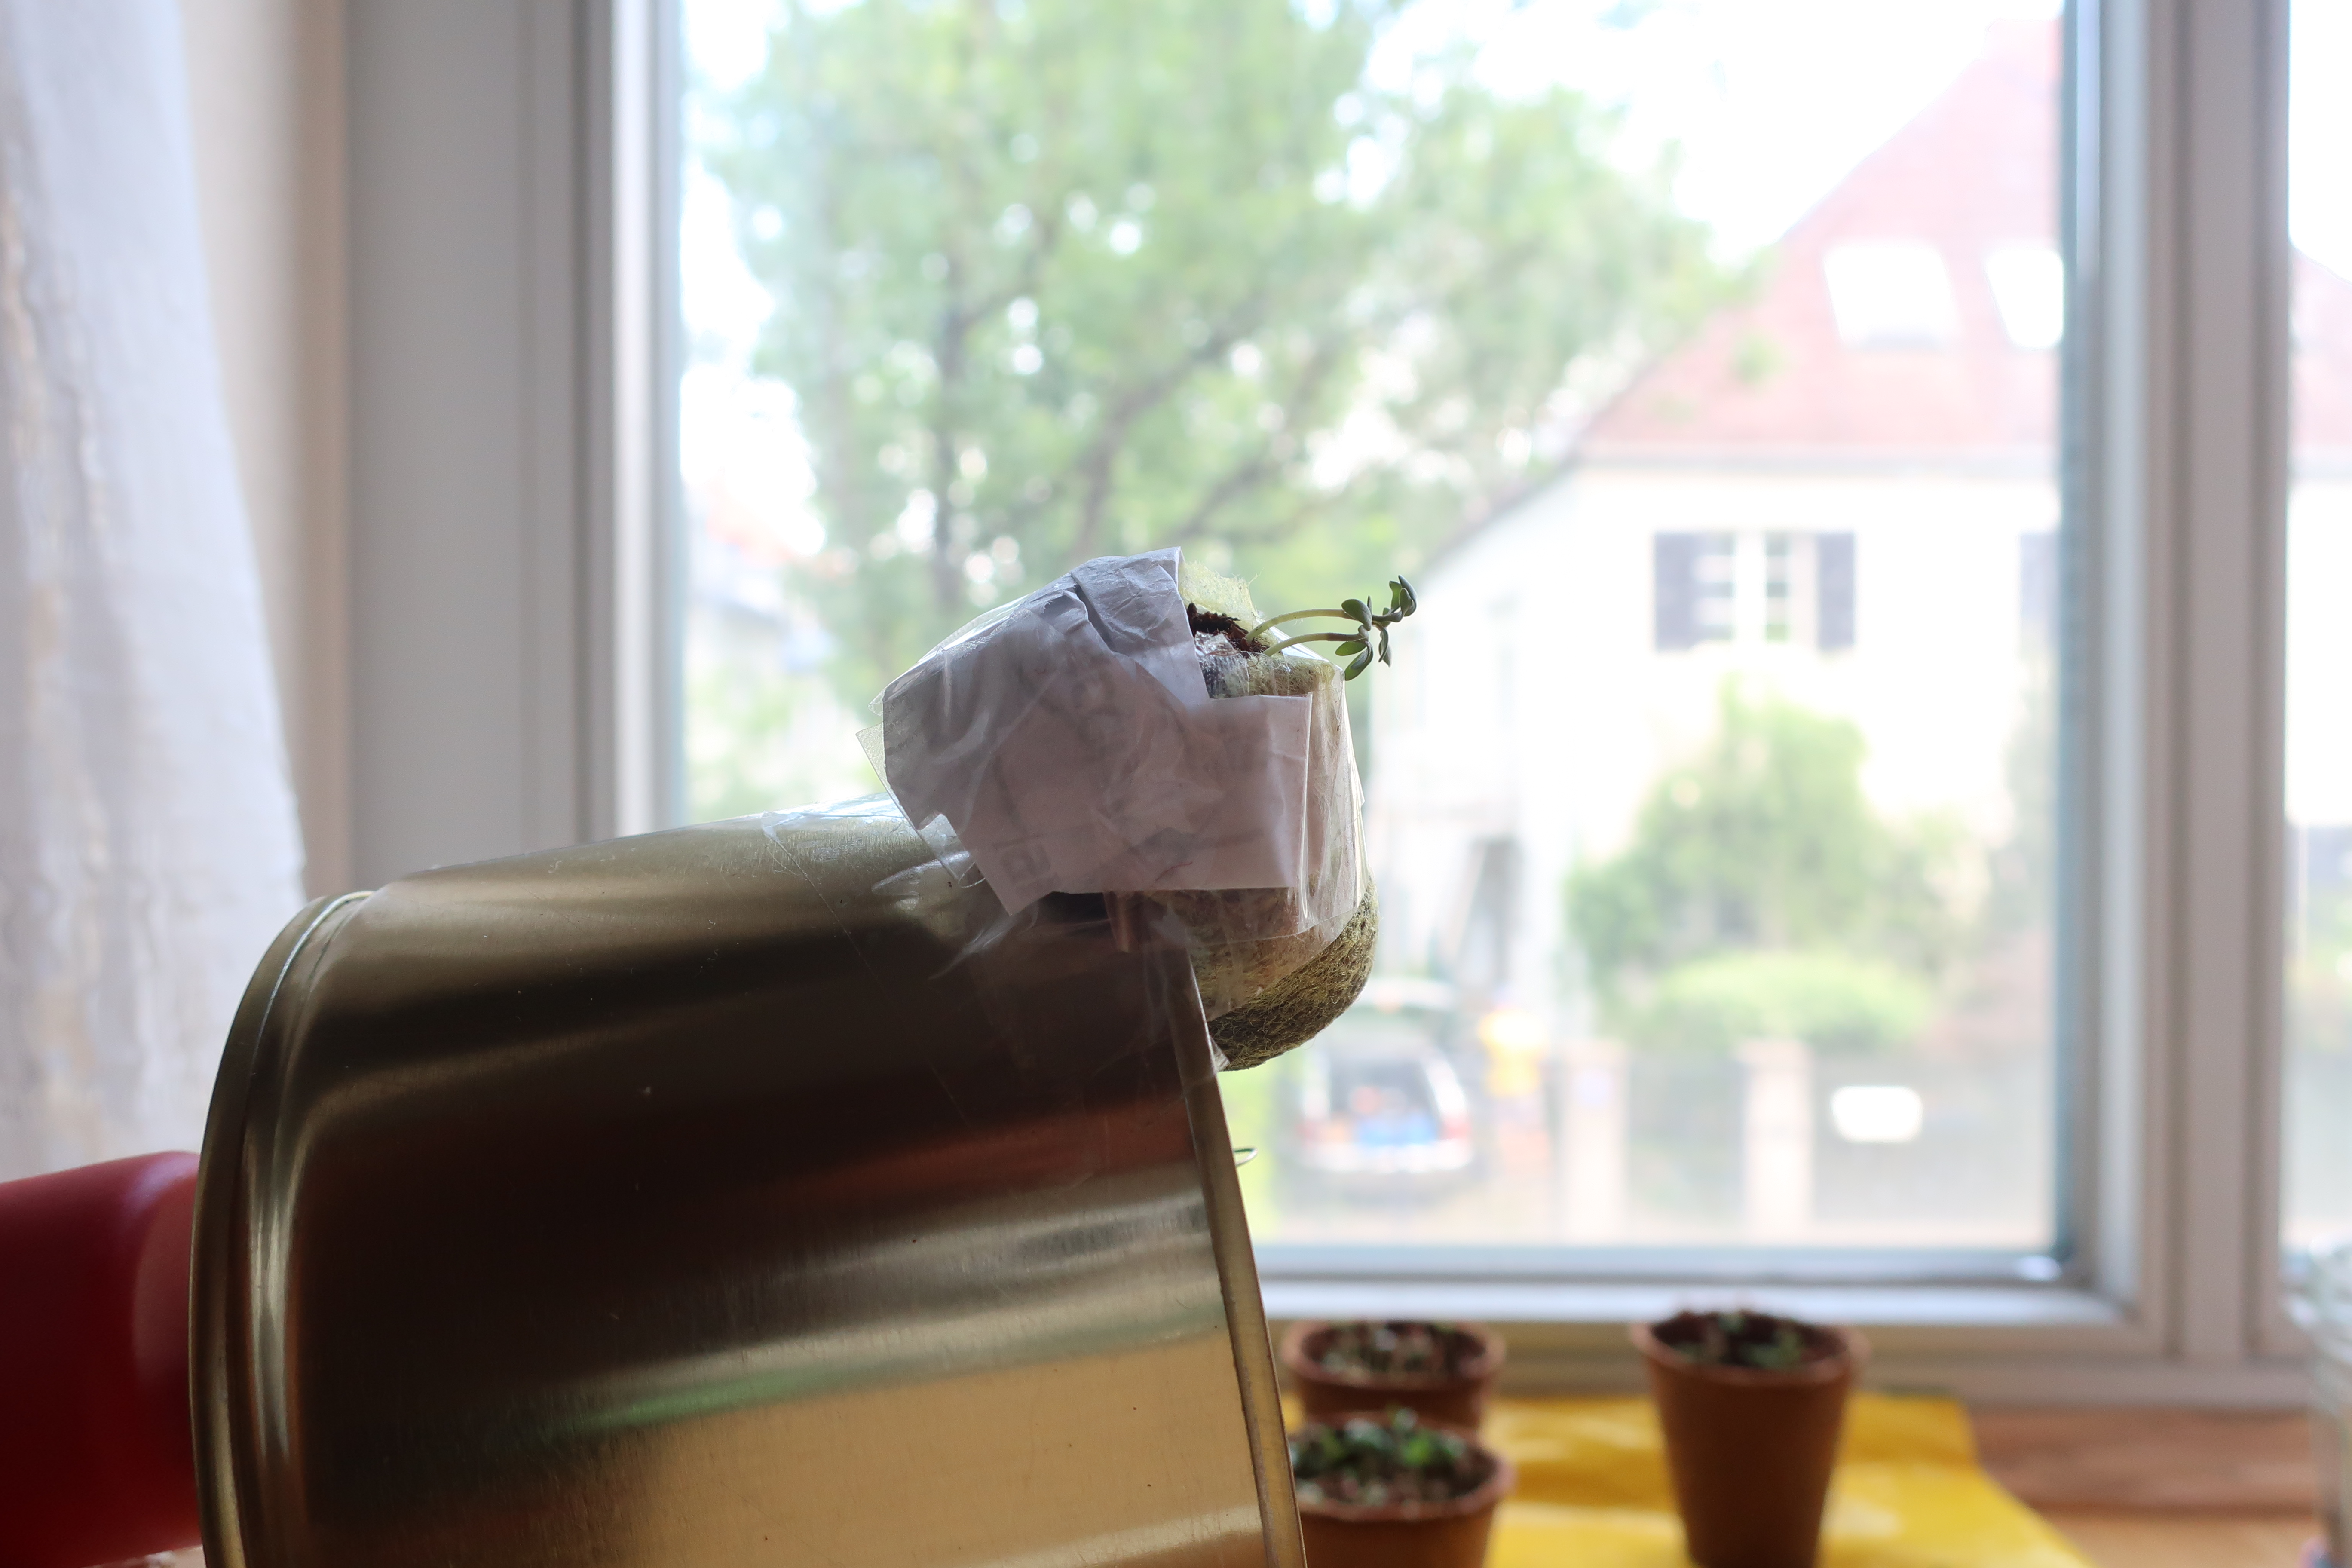
\includegraphics [width = .5\linewidth]{images/IMG_1073.JPG}
%  \end {figure} 
% Photo 2

%\begin{figure}
	%  \centuring 
	%  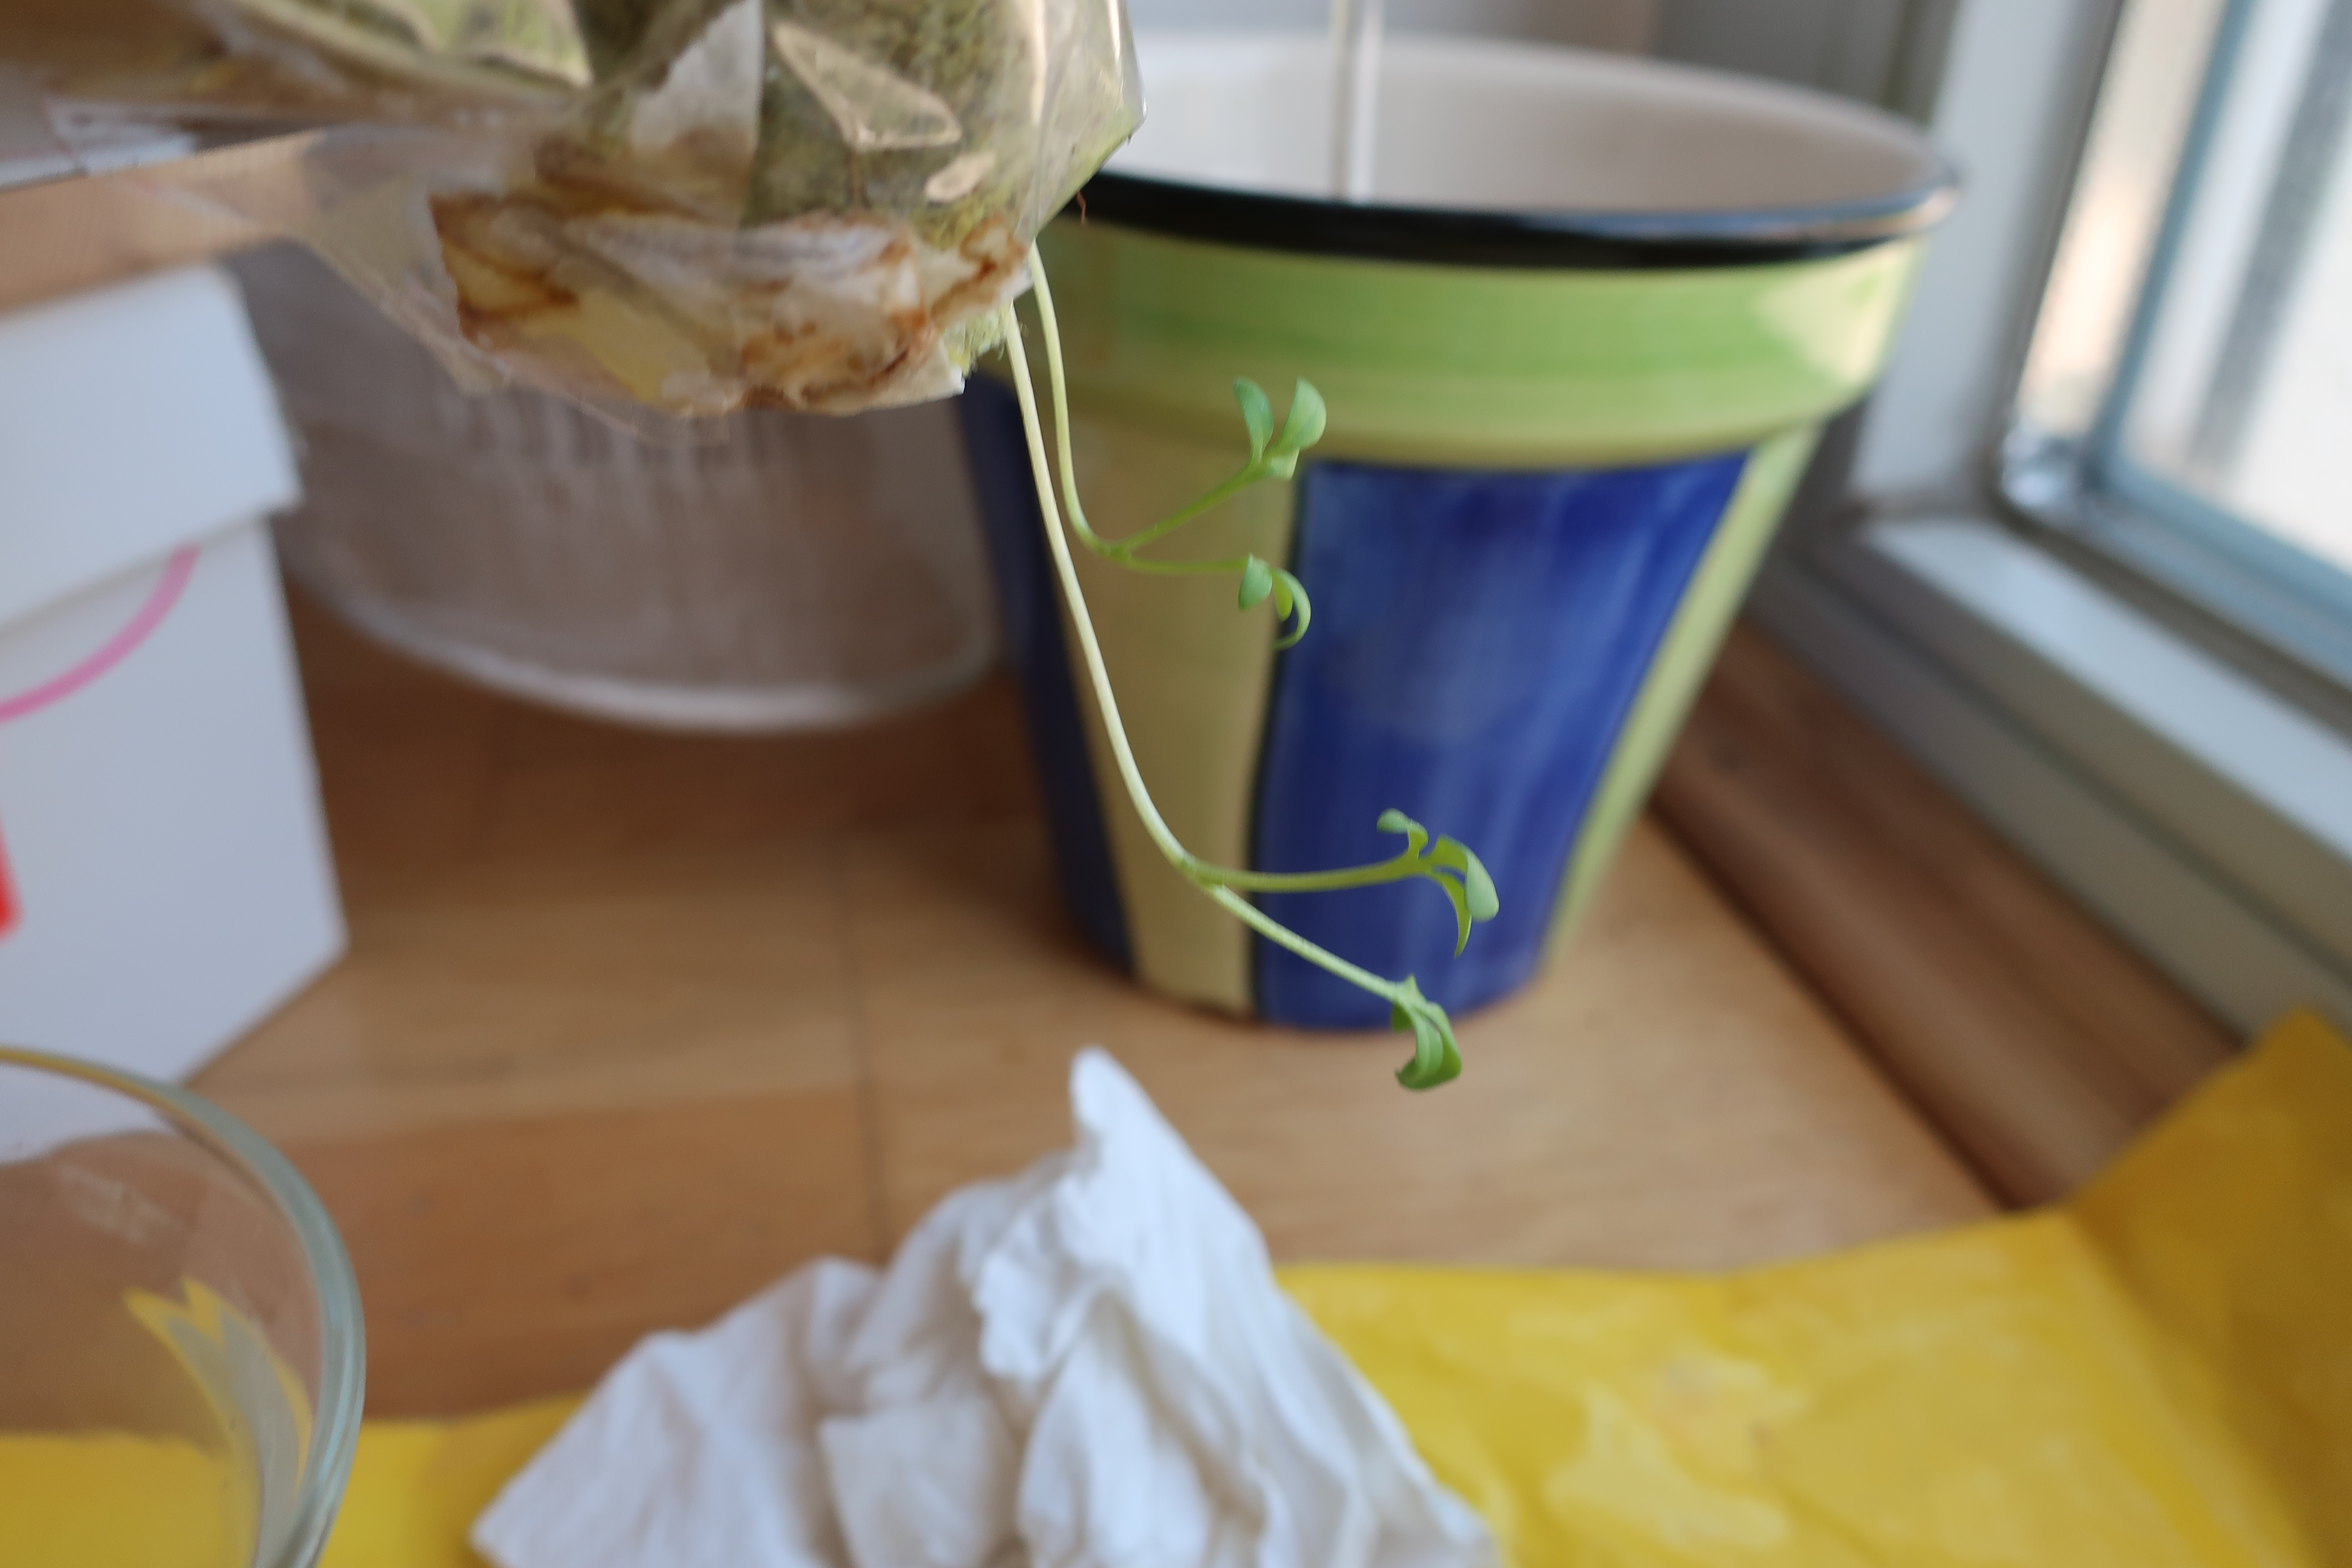
\includegraphics [width =.5\linewidth]{images/IMG_1399.JPG}
	%  \end {figure} 
	% Photo 5

\end{document}
